%======================================================================
%   Zak Webb
%   Ph.D. Thesis
%   Department of Physics and Astronomy
%   University of Waterloo
% 
%   Universality of multi-particle scattering
%======================================================================


\documentclass[../thesis-main/thesis-main]{subfiles}
\begin{document}

\chapter{Universality of multi-particle quantum walk}
\label{chap:MP_universality}



So far in this thesis, we have managed to gain an understanding of single-particle scattering in graphs, which we were then able to use to show the universality of the quantum walk framework for quantum computations.  We have a similar result in \chap{MPQW} for understanding simple multi-particle quantum walk, and thus we will want to understand how such systems can be put together to construct a universal quantum simulator.

The main idea of the construction is very similar to that of \chap{SP_universality}; we encode the computational state in a traveling wavepacket, using the ideas of graph scattering in order to implement single-qubit gates.  The difference, however, is that we encode each qubit with its own particle, thus allowing for much smaller graphs at the expense of more complicated multi-gate behavior.   


At this point, we understand the time-evolution of single particle wave-packets on graphs with long paths, via \thm{single_particle_wavepacket_bound}, and we understand the time-evolution of two particle wave-packets traveling toward each other along a long path, via \thm{two_particle_wavepacket_bound}.  Combining these results, along with the \lem{truncation}, will allow us to understand multi-particle scattering on relatively complicated graphs.  We can then use this understanding to encode computation in the time evolution of initially separate wave-packets.  Note that this idea of encoding qubits in the location of particles was originally used in \cite{Chi09}, but the dual-rail encoding originally occured in \cite{MPQW}.

%%%%%%%%%%%%%%%%%%%%%%%%%%%%%%%%%%%%%%%%%%%%%%%%%%%%%%%%%%%%%%%%%%%%%%%%%%
%  Qubit Encodings
%

\section{Qubit Encoding}

As is \chap{SP_universality}, the first step for simulating a given quantum circuit will be to encode the Hilbert space to be simulated.  In \chap{SP_universality}, we were able to do this by having a number of (nearly) infinite paths equal to the dimension of the Hilbert space,  where the encoded state corresponded to the path on which the particle was located.  While this construction works, the fact that the number of paths grows exponentially in the number of encoded qubits makes this impractical for actually constructing a physical system with a quantum walker.

However, for a small number of basis states, this construction is simple and technically feasible.  The problem of exponential growth arises from the necessary growth of the Hilbert space, since having a larger number of paths was the only means of adding states to the scattering space.  However, when we allow the addition of multiple particles, this then becomes an avenue for increasing the Hilbert space as well.

As such, our encoding of a single-qubit will be identical to that of \chap{SP_universality}; with some specific momenta chosen $k$, we encoded the value of the qubit in a dual-rail encoding.  The value of the encoded qubit will be $\ket{0}$ if the particle is located along the first (top) path, while the value of the encoded qubit will be $\ket{1}$ if the particle is located along the second (bottom) path.

To expand our encoding to multiple qubits, we then add additional paths, but we also add additional particles.  Namely, for each additional qubit, we add two paths and a single particle with some momentum $k_i$.  Again, for that qubit, the value of the encoded qubit is $\ket{0}$ if the particle is located along the top path, wile the value of the qubit will be $\ket{1}$ if the particle moves along the bottom path.

Note that each qubit has its own momentum: while we could require each particle to be encoded at the same momentum, our eventual construction of a multi-qubit entangling gate requires at least two different momenta.  Because of this, we will label each qubits momentum $k_i$, but we will eventually have that most will be equal to some particular value.  One problem that this will lead to is a possible difference in speeds; given the fact that the momenta is explicitly related to the speed of propagation for a given wave-packet, we will need to ensure that the wave-packets move together through the graph.

With the general idea for the encodings out of the way, we will need to explicitly define our states.  In particular, for each qubit we want to simulate, let us assume that there are two infinite paths, where the vertices are labeled as $(x,z,i)$, for $x\in \ZZ$, $z\in \FF_2$ and $i\in[n]$.  Note that the infinite assumption won't be necessary 

Recall from \chap{SP_u} and \chap{MPQW} that for a given $\sigma$, cutoff length $L$, and momentum $k$, we defined the state
\begin{align}
  \ket{\chi_{\mu,k}} = \gamma \sum_{\mu - L}^{\mu + L} e^{ikx} e^{-\frac{(x-\mu)^2}{2\sigma^2}} \ket{x},
\end{align}
and we used states of this form as our assumed wave-packets.  We will use similar states for our encoded qubits, where $\sigma$ and $L$ will depend on the overall length of the computation.  Moreover, we will use the same $L$ and $\sigma$ for all of the qubits.

In particular, we will then say that a logically encoded basis state $\ket{\mathbf{z}}$ for $\mathbf{z}\in \FF_2^n$ will be encoded in the state
\begin{align}
  \ket{\mathbf{z}}_{\text{log}} &= \bigotimes_{j\in [n]} \sum_{\mu_j-L}^{\mu_j+L} e^{i k_j x} e^{- \frac{(x - \mu_j)^2}{2\sigma^2}} \ket{x,z_j,j},
\end{align}
with the rest of the Hilbert space defined in a linear manner.  Note that each individual qubit has its own momentum $k_i$ and position $\mu_i$.  



\subsection{Single qubit gate simulation}

Now that we have encoded qubits, we will want to know how to apply a single particle gate.  For a single qubit, this will be done exactly as in \chap{SP_universality}.  Namely, for a given qubit with momentum $k$, if we want to apply the unitary $U$, we will place a graph $\widehat{G}$ as an obstacle along the pair of infinite paths, where the scattering matrix at $k$ of $\widehat{G}$ takes the form
\begin{align}
  S(k) = \begin{pmatrix}
    0& U^T\\
    U & 0
  \end{pmatrix}
\end{align}
where we assume that the labeling of the four terminal vertices proceeds as $0_{\text{in}}$, $1_{\text{in}}$, $0_{\text{out}}$, and $1_{\text{out}}$, as in \todo{figure something}. 

When we add additional qubits, however, things differ from the single-particle case.  In \chap{SP_u}, in the case of $n$ qubits, each single-qubit gate required $2^{n-1}$ copies of the graph gadget $\widehat{G}$ in order to implement the logical gate.  For the multi-particle encoding, only a single copy of the graph is placed as an obstacle on the pair of paths corresponding to the qubit on which the gate is applied, while the rest of the qubits simply remain unimpeded.  

\subsection{Finite graphs for single-qubit gates}

\todo{fix}

While an understanding of the scattering behavior for infinite graphs is useful to give a broad overview of the dynamics, we will eventually need to restrict ourselves to finite sized graphs.  In particular, we will restrict ourselves exactly as in the case for single-particle scattering in \chap{SP_universality}.

Moreover, we will actually be able to use \lem{single_qubit_encoded_computation}, as in our encoded logical states, each individual particle is located on a separate component of the underlying graph, so that the evolution is exactly that of free particles.  Basically, we have that for all times the particles remain an infinite distance apart, and thus will never interact.  As the evolution then decomposes into a product of evolutions for each individual particle, the results of \lem{single_qubit_encoded_computation} will follow.  In particular, we will be able to use \lem{disconnected_MPQW} to evolve each particle independent of the other using the approximations of \lem{single_qubit_encoded_computation}, and see that the errors add linearly.

In particular, let us assume that a given graph $G$ has $M$ components, and let us assume that $\ket{\psi}$ is an $N$ particle state with support only on multi-particle states where each particle is located on separate components

Namely, let us assume that we want to apply a single-qubit gate $U$ to qubit $j$, where there exists a gadget $\widehat{G}$ that implements this unitary at momentum $k_j$.  Further, let us assume that the wave-packet for qubit $j$ is located a distance $\mu_j$ from the scattering gadget.  If we then assume that each qubit's wave-packet corresponds is located at a position $\mu_j$, where the 


\begin{figure}
  \centering  
  \tikzsetnextfilename{MP_u_sqf}
  \input{../tikz/MP_u_sqf.tex}
  \caption{A block of type I. Here the single-qubit gates $U_1,\ldots,U_n$ on the encoded computational qubits are either the phase gate, the basis-changing gate, or the identity (up to a global phase). The single-qubit gate $V_\med$ on the mediator is either the identity or the Hadamard gate (again, up to a global phase).}
\label{fig:MP_u_sqf}
\end{figure}

\subsection{Many particle simulation}

\todo{this}

While our previous results give us a good understanding of the 

%%%%%%%%%%%%%%%%%%%%%%%%%%%%%%%%%%%%%%%%%%%%%%%%%%%%%%%%%%%%%%%%%%%%%%%%%%
%  Applying an encoded C\theta gate
%

\section{Entangling gate}


Now that we have encoded qubits and, at specific momenta, a universal set of single-qubit gates, we need to construct some kind of entangling gate between our encoded qubits.  In the single-particle encoding, this gate was trivial, as a controlled-not gate (and in fact any permutation gate) simply corresponded to a relabelling of the encoding paths.  For our multi-particle encoding, however, the entanglement procedure is rather more involved.  Our entangling gate will necessarily involve a two-particle Hamiltonian, but we will arrange the graph (and the encoded states) in such a manner that the two-particles will only ever interact on a (long) path.  As such, we can use \thm{two_particle_wavepacket_scattering} to see that the result of such scattering is simply an applied phase.  

Explicitly, our entangling gate will be a controlled-$\theta$ gate, for some $\theta$ that depends on the interaction and the momenta used to encode the qubits.  Further, our entangling gate will only exist between qubits that are encoded with particles for which a momentum switch \sec{mom_switch} exists, which necessitates the use of at least two different momenta.  The main idea behind the gate is to place two momentum switches (represented schematically as \fig{mom_switch}) on the $1$-paths of the qubits as obstacles, where the two switches are connected by a long path for their third terminals.  In either particle is in the logical state $1$, it will be routed along the long connecting path between the two paths, and then routed along $1_{\text{out}}$ for the opposite qubit.  By arranging the lengths of the various paths correctly, we can ensure that if at most a single encoded qubit is in the logical $1$ state, then the corresponding single-particle scattering events encode identity operations.  However, if both encoded qubits are logically $1$, then the two particles move past each other along the long connecting path, acquiring an additional phase that depends on their momenta and the interaction.  As such, the graph in \fig{cd_gate} applies an encoded $\CD$ gate.


\begin{figure}
\centering
\subfloat[][]{
  \tikzsetnextfilename{MP_u_mom_switch}
  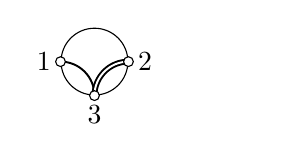
\begin{tikzpicture}
  [ scale = 0.6,
    thin,
    inner/.style={circle,draw=black!100,fill=black!100,inner sep=1.25pt},
    attach/.style={circle,draw=black!100,fill=black!0,thin,inner sep=1.25pt},
    sin/.style={line width=.7pt},
    doub/.style={line width=2.1pt},
    trip/.style={draw=white,line width=.7pt}]
    \node at (0,0){};
%\begin{scope}[yshift=1.8cm]
%  \node (2)  at (0,0) [attach,label=left:3] {};
%  \node (1)  at (0,1) [attach,label=left:1] {};
%  \node (3)  at (3,1) [attach,label=right:2] {};
%  \node (4)  at (1,0) [inner]  {};
%  \node (5)  at (2,0) [inner]  {};
%  \node (6)  at (1,1) [inner]  {};
%  \node (7)  at (2,1) [inner]  {};
%  \node (8)  at (2,2) [inner]  {};
%  \node (9)  at (2.866,2.5)  [inner] {};
%  \node (10) at (1.134,2.5)  [inner] {};
%  \node (11) at (2,-1)       [inner] {};
%  \node (12) at (2.866,-1.5) [inner] {};
%  \node (13) at (1.134,-1.5) [inner] {};
%
%  \draw (2) to (4);
%  \draw (4) to (5);
%  \draw (3) to (7);
%  \draw (1) to (6);
%  \draw (6) to (4);
%  \draw (6) to (7);
%  \draw (7) to (5);
%  \draw (7) to (8);
%  \draw (8) to (9);
%  \draw (8) to (10);
%  \draw (11) to (5);
%  \draw (11) to (12);
%  \draw (11) to (13);
%
  \node (split) at (-3.6,.8) [draw=black,circle,inner sep=3mm,
         label=left:1,label=right:2,label=below:3] {};
% 
%  \node at (-1.6,.5) {=};

  \draw[sin]  (split.west) to[out=0,in=90]   (split.south);
  \draw[doub] (split.east) to[out=180,in=90] (split.south);
  \draw[trip] (split.east) to[out=180,in=90] (split.south);
  
  \node at (split.east) [attach] {};
  \node at (split.west) [attach] {};
  \node at (split.south) [attach]{};
%\end{scope}
\end{tikzpicture}
  \label{fig:mom_switch}
}
\hspace{0.5cm}
\subfloat[][]{
  \tikzsetnextfilename{MP_u_cd_gate}
  \begin{tikzpicture}
  [ scale = 1,
    yscale = .8,
    attach/.style={circle,draw=black!100,fill=white,thick,
    minimum size = 6mm},
    cross/.style={line width=4pt, draw=white},
    drawn/.style={draw=black},
    vert/.style = {circle,fill=black,inner sep=.6pt, minimum size=0},
    nofill/.style = {circle,draw=black,fill=white,inner sep = 1.25pt,minimum size=0},
    decoration={markings,
		mark=between positions 0 and 10 step .1cm
 		with { \node at (0,0) [vert]{}; }}]

  \node (bottom) at ( 1, 0) [attach] {};
  \node (top)    at ( 1, 2.5) [attach] {};
  
  \foreach \x in {0,.1,...,3.5}{
  \foreach \y in {.75, 3.25}{
    \node at (\x,\y) [vert] {};
  }}

  \draw[postaction={decorate}] (0,0) node[left] {$1_{\med,\text{in}}$} 
    -- (bottom.west);
  \draw (0,.75) node [left] {$0_{\med,\text{in}}$} 
    -- (3.5,.75) node [right] {$0_{\med,\text{out}}$};
  \draw (0,3.25) node [left] {$0_{c,\text{in}}$}
    -- (3.5,3.25) node [right] {$0_{c,\text{out}}$};
  \draw[postaction={decorate}] (0,2.5) node [left] {$1_{c,\text{in}}$} 
    -- (top.west) ;
  \draw (top.south) -- (bottom.north) [cross];

  \draw (top.south) -- (bottom.north) [drawn,postaction={decorate}];
  \draw (top.east) -- ( 2, 2.5)  .. controls (2.5,2.5) and (2.5, 0) 
                   .. (3,0) -- (3.5, 0)  [cross];
  \draw (top.east) -- ( 2, 2.5)  .. controls (2.5,2.5) and (2.5, 0) 
                    .. (3,0) -- (3.5, 0) 
                    node [right] {$1_{\med,\text{out}}$} [drawn,postaction={decorate}];
  \draw (bottom.east) -- ( 2, 0) .. controls (2.5,0) and (2.5,2.5)  
                      .. (3,2.5) -- (3.5, 2.5)  [cross];
  \draw[drawn,postaction={decorate}] (bottom.east) -- ( 2, 0) .. controls (2.5,0) and (2.5,2.5)  
                      .. (3,2.5) -- (3.5, 2.5) 
                      node [right] {$1_{c,\text{out}}$} ;

  \draw (top.west) to[out=0,in=90] (top.south) [line width = .7pt];
  \draw (bottom.east) to[out=-180,in=-90] (bottom.north) [line width=.7pt];
  \draw (top.east) to[out=-180,in=90] (top.south) [line width=2.1pt];
  \draw (top.east) to[out=-180,in=90] (top.south) [line width=.7pt,draw=white];
  \draw (bottom.west) to[out=0,in=-90] (bottom.north) [line width=2.1pt];
  \draw (bottom.west) to[out=0,in=-90] (bottom.north) [line width=.7pt,draw=white];  
  
  
  \foreach \x in {0, 3.5}{
  \foreach \y in {0,.75, 2.5, 3.25}{
    \node at (\x,\y) [nofill] {};
  }}
 
 \node at (top.west) [nofill]{};
 \node at (top.east) [nofill]{};
 \node at (top.south) [nofill]{};
 \node at (bottom.west) [nofill]{};
 \node at (bottom.east) [nofill]{};
 \node at (bottom.north) [nofill]{};
  
\end{tikzpicture}
  \label{fig:cd_gate}
}
\caption{\subfig{mom_switch} Momentum switch schematic. \subfig{cd_gate} $\CD$ gate.}
\label{fig:onepsplit}
\end{figure}

\subsubsection{Momentum switch}

Remember from \sec{mom_switch} that momentum switches are three-terminal scattering gadgets that act like railroad switches, where at specific momenta the gadget has perfect transmission from terminal 3 to terminal 1, while at other momenta there is perfect transmission from terminal 3 to terminal 2.  We will represent gadgets with this behavior schematically as in \fig{mom_switch}, where one set of momenta follow the single line while the other specified set follows the double line.

For our purposes, we will assume that the momentum switch splits the two momenta used to encode the different qubits $k_{1}$ and $k_{2}$.  Explicitly, we will assume that the $S$-matrix for the given momentum switch at $k_1$ and $k_2$ are given by
\begin{equation}
  S_{\text{switch}}(k_{1}) = \begin{pmatrix} 0 & 0 & T_{1}\\
    0 & R_{1} & 0\\
    T_{1} & 0 & 0\end{pmatrix}\qquad
  S_{\text{switch}}(k_{2}) = \begin{pmatrix}R_{2} & 0 &0\\
    0 & 0 & T_{2}\\
    0 & T_{2} & 0\end{pmatrix}.
\label{eq:switch_S}
\end{equation}
In other words, we will assume that the momentum switch has perfect transmission between terminals $1$ and $3$ at momentum $k_{1}$, and perfect transmission between terminals $2$ and $3$ at momentum $k_{2}$, possibly with an additional phase.  With this, we have that a particle with momentum $k_{1}$ follows the single line of the schematic representation of \fig{mom_switch}, while a particle with momentum $k_{2}$ follows the double line.


\subsubsection{Constructing the graph}

We will now construct this graph, where we will assume that we know the encoded initial states.  Note that this construction doe depend on the momenta of the encoded qubits in more than just the form of the momentum switch; the fact that the timing of the wave-packets is important forces us to change the length of the connecting paths depending on the initial momentum so that they arrive on the infinite path at the same time, while the requirement that the particles only interact along the path forces us to change the lengths depending on the size of the wave-packets.

The $\CD$ gate is implemented using the graph shown in \fig{explicit_cd}. In this section we specify the logical input states, the logical output states, the distances $X$, $Z$, and $W$ appearing in the figure, and the total evolution time as functions of the momentum $k_{1}$ and $k_{2}$. With these choices, we show that a $\CD$ gate is applied to the logical states at the end of the time evolution under the quantum walk Hamiltonian (up to error terms that are $\tilde{\O}(L^{-{1}/{2}})$). The results of this section pertain to the two-particle Hamiltonian $H^{(2)}_{G'}$ for the graph $G'$ shown in \fig{explicit_cd}.
\todo{get correct error term}

\begin{figure}
  \centering
  \tikzsetnextfilename{MP_u_explicit_cd}
  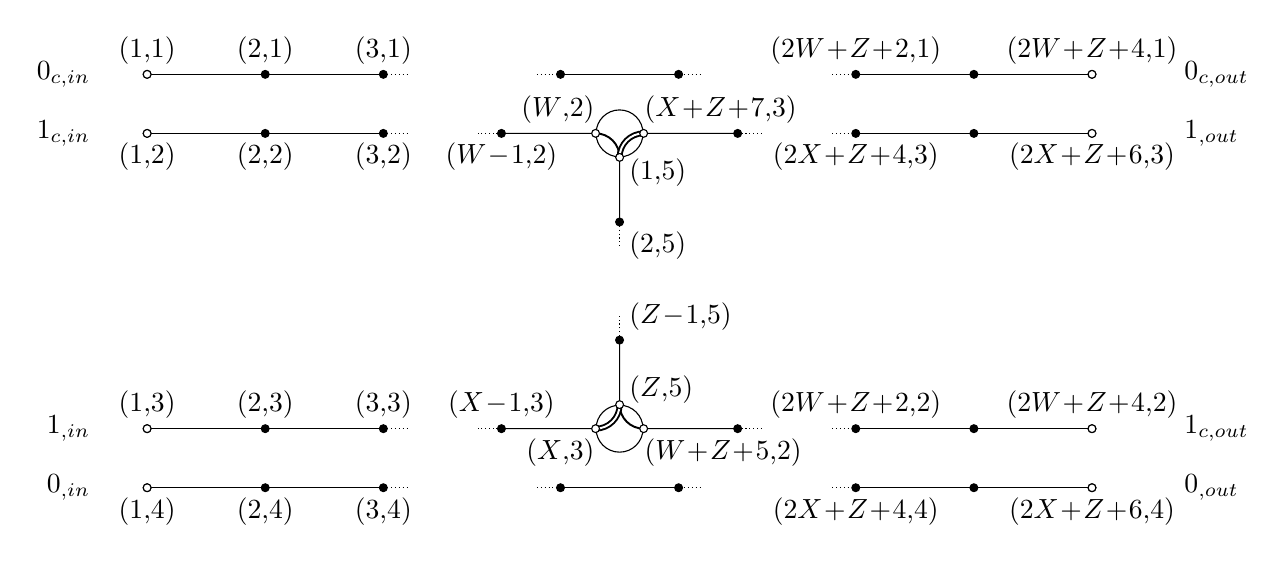
\begin{tikzpicture} [scale=1.5,
	vert/.style={circle, draw=black, fill=black,inner sep=1pt, minimum width=0pt},
	dots/.style={circle, fill=black,inner sep=1pt, minimum width=0pt},
	switch/.style={circle,draw=black,inner sep=6pt,minimum width=0pt},
	attach/.style={circle,fill=white, draw=black,inner sep=1pt, minimum width=0pt}]

  \foreach \y in {0,0.5,3,3.5}{
  \begin{scope}[yshift=\y cm]
  \foreach \x in {0,1,2,6,7,8}{
	\begin{scope}[xshift = \x cm]
	  \node at (0,0) [vert]{};
	\end{scope}}
	\draw (0,0) -- (2,0);
	\draw (6,0) -- (8,0);
	\draw[densely dotted] (2,0)--(2.2,0);
	\draw[densely dotted] (5.8,0)--(6,0);
	\node at (0,0) [attach] {};
	\node at (8,0) [attach] {};
 \end{scope}}
 
  
  \node (switch2) at (4,0.5)[switch]{};
  \node (switch1) at (4,3)[switch]{};
  
  \node at (3,0.5) [vert]{};
  \node at (3,3) [vert]{};
  \node at (5,0.5) [vert]{};
  \node at (5,3) [vert]{};
  
  \draw (switch2.west) -- (3,0.5);
  \draw[densely dotted] (3,0.5) -- (2.8,0.5);
  \draw (switch2.east) -- (5,0.5);
  \draw[densely dotted] (5,0.5) -- (5.2,0.5);
  
  \draw (switch1.west) -- (3,3);
  \draw[densely dotted] (3,3) -- (2.8,3);
  \draw (switch1.east) -- (5,3);
  \draw[densely dotted] (5,3) -- (5.2,3);
  
  \node at (3.5,0) [vert]{};
  \node at (4.5,0) [vert]{};
  \node at (3.5,3.5) [vert]{};
  \node at (4.5,3.5) [vert]{};
  
  \draw (3.5,0) -- (4.5,0);
  \draw (3.5,3.5) -- (4.5,3.5);
  \draw[densely dotted] (3.3,0) -- (4.7,0);
  \draw[densely dotted] (3.3,3.5) -- (4.7,3.5);
  

  \node at (4,1.25) [vert] {};
  \node at (4,2.25) [vert] {};
  
  \draw (switch2.north) -- (4,1.25);
  \draw[densely dotted] (4,1.25) -- (4,1.45);
  
  \draw (switch1.south) -- (4,2.25);
  \draw[densely dotted] (4,2.25)-- (4,2.05);
  
  \draw[line width=.7pt] (switch1.west) to[out=0,in=90] (switch1.south);
  \draw[line width=2.1pt] (switch1.east) to[out=180,in=90] (switch1.south);
  \draw[line width=.7pt,white] (switch1.east) to[out=180,in=90] (switch1.south);

  \draw[line width=.7pt] (switch2.east) to[out=180,in=-90] (switch2.north);
  \draw[line width=2.1pt] (switch2.west) to[out=0,in=-90] (switch2.north);
  \draw[line width=.7pt,white] (switch2.west) to[out=0,in=-90] (switch2.north);
  
  \node at (switch2.north) [attach] {};
  \node at (switch1.south) [attach] {};
  \node at (switch2.east) [attach] {};
  \node at (switch1.east) [attach] {};
  \node at (switch2.west) [attach] {};
  \node at (switch1.west) [attach] {};
  
  \node at (0,0) [below] {(1,4)};
  \node at (1,0) [below] {(2,4)};
  \node at (2,0) [below] {(3,4)};
  \node at (3.5,0) [below] {};
  \node at (4.5,0) [below] {};
  \node at (6,0) [below] {($2X\!+\! Z\! + \! 4$,4)};
  \node at (8,0) [below] {($2X\! +\! Z\! +\! 6$,4)};
  
  \node at (0,3.5) [above] {(1,1)};
  \node at (1,3.5) [above] {(2,1)};
  \node at (2,3.5) [above] {(3,1)};
  \node at (3.5,3.5) [above] {};
  \node at (4.5,3.5) [above] {};
  \node at (6,3.5) [above] {($2W\! + \! Z\! + \! 2$,1)};
  \node at (8,3.5) [above] {($2W\! + \! Z\! + \! 4$,1)};
  
  \node at (0,3) [below] {(1,2)};
  \node at (1,3) [below] {(2,2)};
  \node at (2,3) [below] {(3,2)};
  \node at (3,3) [below] {($W\!-\! 1$,2)};
  \node[anchor=south east] at (3.87,3) {($W$,2)};
  
  \node at (0,.5) [above] {(1,3)};
  \node at (1,.5) [above] {(2,3)};
  \node at (2,.5) [above] {(3,3)};
  \node at (3,.5) [above] {($X\! -\! 1$,3)};
  \node at (3.87,.5) [below left] {($X$,3)};
  
  \node at (8,.5) [above] {($2W\! + \! Z\! + \! 4$,2)};
  \node at (6,.5) [above] {($2W\! + \! Z\! + \! 2$,2)};
  \node at (4.13,.5) [below right] {($W\! + \! Z\! + \! 5$,2)};  
  
  \node at (8,3) [below] {($2X\! + \! Z\! + \! 6$,3)};
  \node at (6,3) [below] {($2X\! + \! Z\! + \! 4$,3)};
  \node at (4.13,3) [above right] {($X\! + \! Z\! + \! 7$,3)};
  
  \node at (4,2.87) [below right] {(1,5)};
  \node at (4,2.25) [below right] {(2,5)};
  
  \node at (4,.63) [above right] {($Z$,5)};
  \node at (4,1.25) [above right] {($Z\! -\! 1$,5)};
  
  \node at (-.4,0) [left] {$0_{\med,\text{in}}$};
  \node at (-.4,.5) [left] {$1_{\med,\text{in}}$};
  \node at (-.4,3) [left] {$1_{c,\text{in}}$};
  \node at (-.4,3.5) [left] {$0_{c,\text{in}}$};
  
  \node at (8.7,0) [right] {$0_{\med,\text{out}}$};
  \node at (8.7,.5) [right] {$1_{c,\text{out}}$};
  \node at (8.7,3) [right] {$1_{\med,\text{out}}$};
  \node at (8.7,3.5) [right] {$0_{c,\text{out}}$};
\end{tikzpicture} 
  \caption{Graph $G'$ used to implement the $\CD$ gate. The integers $Z$, $X$, and $W$ are specified in equations \eq{Z_eq}, \eq{X_eq}, and \eq{W_eq}, respectively.}
\label{fig:explicit_cd}
\end{figure}

We first need to construct the assumed encoded initial states.  Note that the important bit about these encodings are the length and cutoff distance.  While the distance from the ends, and the distance from the scattering widgets are important, they won't affect the overall qualitative action of the wave-packets.  Additionally, note that the labeling scheme for the vertices is as in \fig{explicit_cd}.  We can then assume that our initial logical states are
\begin{align}
  |0_{\text{in}}\rangle^{1}&=  \gamma \sum_{x = \mu_0 -L} ^{\mu_0 + L}  e^{i k_{1} x} e^{- \frac{(x-\mu_0)^2}{2\sigma^2}} \ket{x,1} & 
  |1_\text{in}\rangle^1&= \gamma \sum_{x = \mu_0 -L} ^{\mu_0 + L}  e^{i k_{1} x} e^{- \frac{(x-\mu_0)^2}{2\sigma^2}} \ket{x,2} \label{eq:cd_input_1}
\end{align}
for the qubit with momentum $k_1$ and
\begin{align}
  |0_{\text{in}}\rangle^2&=\gamma \sum_{x = \nu_0 -L} ^{\nu_0 + L}  e^{i k_{2} x} e^{- \frac{(x-\nu_0)^2}{2\sigma^2}} \ket{x,4}&
  |1_\text{in}\rangle^2&=\gamma \sum_{x = \nu_0 -L} ^{\nu_0 + L}  e^{i k_{2} x} e^{- \frac{(x-\nu_0)^2}{2\sigma^2}} \ket{x,3} \label{eq:cd_input_2}
\end{align}
 for the qubit with momentum $k_2$.  Additionally, let us assume that $|\sin k_1| \leq |\sin k_2|$, so that the wave-packet with momentum $k_1$ travels no faster than the wave-packet with momentum $k_2$ (this assumption is without loss of generality as we can simply relabel $k_1$ and $k_2$).
 
 Note that the two computational basis states for each qubit are centered at the same distance from the ends, but that the distances are different for the two qubits.  The reason for this is that while the wave-packets for each individual qubit travel at the same speed, differing qubits will most likely travel at unique speeds and we will want to ensure that this is taken care of when we combine these gadgets.
 
 \todo{talk about symmetrized states?}
 %We can then define symmetrized (or antisymmetrized) logical input states for $a,b\in\{0,1\}$ as
%\begin{align*}
%|a b_{\text{in}}\rangle^{\text{com},\med}_\pm &=\frac{1}{\sqrt{2}} \left(|a_{\text{in}}\rangle^{\text{com}} |b_{\text{in}}\rangle^\med \pm |b_{\text{in}}\rangle^\med|a_{\text{in}}\rangle^{\text{com}}\right).
%\end{align*}

With these initial logical states chosen, note that there are seven path lengths that we will need to determine before we can analyze the propagation.  Explicitly, there is the distance on path $2$ corresponding to the initial distance the wave-packet with momentum $k_1$ travels before hitting the first momentum switch, the same for path $3$ and the wave-packet with momentum $k_2$, the distance between the two momentum switches where the two-particles will interact, the lengths of the two output paths after the second momentum switches, and finally the two paths corresponding to the logical states $0$.  Note that these final two path lengths (corresponding to the logical $0$ states) will be determined by the total distance traveled by the logical $1$ states, and that we can assume that the distances after the momentum switch are the same as the distances before the momentum switches.  As such, there are three distances that we care about.

\todo{double check these numbers}

Putting this together, we will need to chose the three distances $Z$, $X$, and $W$ from \fig{explicit_cd} to ensure that we can analyze the wave-packet propagation, while also ensuring that the output approximated wave-packets are in agreeing positions.  While this can be somewhat difficult, we will chose these distances to be
\begin{align}
  Z & = \big(7 + 3 \alpha\big) L \label{eq:Z_eq} \\
  X & = 2L + D+M(k_2) \label{eq:X_eq}\\
  W & = 3L + M(k_1) \label{eq:W_eq}
\end{align}
where
\begin{align}
  \alpha &= \frac{ \sin |k_2| - \sin |k_1|}{\sin |k_1| + \sin |k_2|}\\
  D &= \frac{ \sin^2 k_2 - 2 \sin^2 k_1 + 4 \sin k_1 \sin k_2}{\sin k_1 \big( \sin k_1 + \sin k_2\big)} L \\
  M(k_i) & = 2 t_0 \sin |k_i|.
\end{align}
With these choices, a wave packet moving with speed $\sin |k_1|$ travels a distance $Z+4L=(11+ 3\alpha)L$ in approximately the same time that a wave packet moving with speed $k_2$ takes to travel a distance $Z+2D + 2L=(9+3\alpha)L+2D$, since
\begin{align}
  t_{\CD}=\frac{(11 + 3 \alpha)L}{2 \sin |k_1|} \approx\frac{(9 + 3 \alpha)L + 2 D}{2\sin |k_2|}.
  \label{eq:tcd_defn}
\end{align}
Additionally, these distances are chosen so that at time $t_1 = (4 + 3\alpha)L/2\sin |k_1|$, the two particles are both located on the center path, with the wave-packet with momentum $k_1$ a distance $(1 + 3\alpha)L$ from the first momentum switch, the other a distance $L$ from the second momentum switch, and the two wave-packets a distance $L$ apart, and so that at a time $t_2 = t_1 + 6L/(\sin |k_1| + \sin |k_2|)$, the wave-packets have passed each other, but are now the same distance from the other momentum switch.

One point to notice is that the distances $M(k_i)$ are chosen so that the two wave-packets take the same amount of time to reach their initial position if they initially started centered at the end of the paths.  This isn't particularly important, except to allow us to nicely combine this result with other scattering events.

\subsection{Time evolution analysis}

With the graph $G$ well defined for two momenta $k_1$ and $k_2$, we now want to actually analyze the dynamics of the system.  We want to claim that the initial states evolve into encoded logical output states, where the acquired phases correspond to an entangling gate.  In particular, we will want that the evolution of an encoded state on this graph corresponds to some unitary diagonal in the computational basis, in which an additional phase is acquired for the state $\ket{11}$.  While in an ideal case, this will simply be a controlled-$\theta$ gate, in which the applied unitary is the identity for the other three basis states, our graph will also have additional phases corresponding to a product of single-qubit unitaries arising from the transmission coefficients of the two momentum switches.

However, in order to apply an encoded unitary, we will need to have an encoding of the logical output states.  Letting $t_{\CD}$ be as defined in \eq{tcd_defn}, we will have that the encoded output states for each qubit will be 
\begin{align}
  |0_\text{out}\rangle^1 &=\gamma e^{-2it_{\CD}\cos(k_1)}\sum_{x = \mu_1 -L} ^{\mu_1 + L}  e^{i k_{1} x} e^{- \frac{(x-\mu_1)^2}{2\sigma^2}} \ket{x,1}
  \label{eq:cd_output_10}\\
  |1_\text{out}\rangle^1 &=\gamma e^{-2it_{\CD}\cos(k_1)} \sum_{x = \mu_1 -L} ^{\mu_1 + L}  e^{i k_{1} x} e^{- \frac{(x-\mu_1)^2}{2\sigma^2}} \ket{x,2} \label{eq:cd_output_11}\\
  |0_\text{out}\rangle^2 &=\gamma e^{-2it_{\CD}\cos(k_2)} \sum_{x = \nu_1 -L} ^{\nu_1 + L}  e^{i k_{2} x} e^{- \frac{(x-\nu_1)^2}{2\sigma^2}} \ket{x,4} \label{eq:cd_output_20}\\
  |1_\text{out}\rangle^2 &=\gamma e^{-2it_{\CD}\cos(k_2)} \sum_{x = \nu_1 -L} ^{\nu_1 + L}  e^{i k_{2} x} e^{- \frac{(x-\nu_1)^2}{2\sigma^2}} \ket{x,3}\label{eq:cd_output_21}
\end{align}
where  $\mu_1=\mu_0 + \lceil 2t_{\CD} \sin |k_1|\rceil $ and $\nu_{1}=\nu_0 + \lceil 2 t_{\CD}\sin |k_2| \rceil$. Intuitively, these are simply the expected positions of the wave-packets corresponding to the initial logical states after a time $t_{\CD}$, along with the phases acquired form their energies.  

If we note that the input states don't particularly rely on the initial distance from the graph, and that the output states similarly don't rely on the distance from the end, we will be able to easily combine the time evolution on these graphs with the time evolution on other graphs.  Just so long as the initial wave packets start a distance proportional to $L$ away from the ends, and similarly end a distance proportional to $L$ from the ends, we can us \lem{truncation} in order to determine the overall time evolution.

\todo{correct the assumptions for \lem{cd_bounds}}

\todo{should I split this into several lemmas?}

In particular, we have the following lemma:
\begin{lemma}
Let $G'$ be the graph given in \fig{explicit_cd}, where we assume that the initial and final states as defined in \eq{cd_input_1}, \eq{cd_input_2}, and \eq{cd_output_10}-\eq{cd_output_21} only have support on vertices a distance at least $L/3$ from the ends of the truncated paths.  If the momentum switch has transmission coefficient $T_1$ for momentum $k_1$ and transmission coefficient $T_2$ for momentum $k_2$, and if the phase acquired for two particle scattering between momentum $k_1$ and $k_2$ is given by $\theta_{\pm}$ for symmetric and antisymmetric states, then we have the following approximations for the time-evolved states:
\begin{align}
  \left\Vert e^{-iH_{G'}^{(2)}t_{\mathrm{II}}}|00_{\text{in}}\rangle_{\pm}^{1,2}-|00_{\text{out}}\rangle_{\pm}^{1,2}\right\Vert  & = \O(L^{-{1}/{4}})\label{eq:bound00}\\
  \left\Vert e^{-iH_{G'}^{(2)}t_{\mathrm{II}}}|01_{\text{in}}\rangle_{\pm}^{1,2}-T_{2}^2|01_{\text{out}}\rangle_{\pm}^{1,2}\right\Vert  & = \O(L^{-{1}/{4}})\label{eq:bound01}\\
  \left\Vert e^{-iH_{G'}^{(2)}t_{\mathrm{II}}}|10_{\text{in}}\rangle_{\pm}^{1,2}-T_1^2|10_{\text{out}}\rangle_{\pm}^{1,2}\right\Vert  & = \O(L^{-{1}/{4}})\label{eq:bound10}\\
  \left\Vert e^{-iH_{G'}^{(2)}t_{\mathrm{II}}}|11_{\text{in}}\rangle_{\pm}^{1,2} - e^{i\theta_{\pm}}T_1^2T_2^2|11_{\text{out}}\rangle_{\pm}^{1,2}\right\Vert  & = \O(L^{-{1}/{4}}).\label{eq:bound11}
\end{align}
\label{lem:cd_bounds}
\end{lemma}


\begin{proof}
The first three bounds \eq{bound00}, \eq{bound01}, and \eq{bound10} are similar to the proofs of \chap{SP_universality}, since in each case the two particles are supported on disconnected subgraphs and thus we can use \lem{disconnected_MPQW}.  For each of the single-particle scattering events, we can use a strategy similar to \lem{single_qubit_encoded_computation} to bound the error in our time-evolution for the unsymmetrized two-particle states.  To get the bound of \eq{bound11}, the proof strategy will be similar, but we will also need an application of an application of \thm{two_particle_wavepacket_bound} during the times at which both particles are located on the long path.


Let us first understand the single-particle evolutions on the long paths. Note that $t_{\CD} \leq c L$ for some constant $c$, and thus according to \thm{single_particle_wavepacket_bound}, on an infinite path $P$ we have that
\begin{align}
  \bigg\Vert \gamma e^{- i P t } \sum_{\mu-L}^{\mu+L} e^{i k x} e^{-  \frac{(x-\mu)^2}{2\sigma} }\ket{x} - \gamma  e^{-2i t \cos(k)} \sum_{\mu(t) - L}^{\mu(t) + L} e^{ i k x} e^{- \frac{(x-\mu(t))^2}{2\sigma^2}} \ket{x} \bigg\Vert \leq \xi \sqrt{\frac{ \log L}{L}}
\end{align}
for some constant $\xi$ and where $\mu(t) = \mu(t) + \lceil 2 t \sin(k)\rceil$.  While \thm{single_particle_wavepacket_bound} doesn't exactly give us this, if we apply the theorem to a graph gadget $\widehat{G}$ that results in the final graph being a long path, and assume that the initial location is far from the scattering event, the result follows after a relabeling of the basis states.  If we then note that the corresponding approximation involving $\mu(t)$ on the finite path always remains a distance of at least $L/3$ away from the ends of the finite approximation and that the initial state only has support on the component corresponding to the finite path so that the evolution according to $A(G')$ is identical to that of the finite path, \lem{truncation} with $H = A(P)$, $\tilde{H} = A(G')$, and $N_0 = \frac{L}{3}$, and the error bound of $\delta =\xi \sqrt{\log L/L}$ gives us
\begin{align}
  \big\Vert e^{-i A(G') t_{\CD}} \ket{0_{\text{in}}}^i - \ket{0_\text{out}}^i\big\Vert &\leq \bigg( \frac{ 8 e t_{\CD}}{N_0} + 2 \bigg) \bigg[\xi \sqrt{\frac{\log L}{L}} + 2^{- N_0} \bigg( 1 - \xi \sqrt{\frac{\log L}{L}}\bigg)\bigg]\\
  & \leq \zeta \sqrt{ \frac{\log L}{L}}
\end{align}
for some constant $\zeta$ that is independent of the momentum $k$.  Hence, we have that this approximation holds for both long paths.


Now let us analyze the single-particle evolution on the subgraph that connects the two particles.  For both particles, we will define approximations to the time-evolved wave packets that will equal both the initial state and the corresponding final states.  Namely, if we also label the vertices of the path 5 (the one of length $Z$ which are currently labeled $(x,5)$) as $(W+1+x,2)$ and $(X + Z - x+2,3)$, then we can define the states 
\begin{align}
  \ket{\alpha_{1}^1(t)} &= \gamma e^{-2 i t \cos(k_1)} \sum_{x = \mu(t) - L}^{\mu(t) + L} e^{ i k_1 x} e^{-\frac{(x-\mu(t))^2}{2\sigma^2}} \ket{x,2}\\
  \ket{\alpha_{2}^1(t)} &= \gamma e^{-2 i t \cos(k_2)} \sum_{x = \nu(t) - L} ^{\nu(t) + L} e^{i k_2 x} e^{-\frac{(x-\nu(t))^2}{2\sigma^2}} \ket{x,3}
\end{align}
where $\mu(t) = \mu + \lceil 2 t \sin (k_1)\rceil$ and $\nu(t) = \nu + \lceil 2 t \sin (k_2)\rceil$.  Note that these are (almost) the same approximations as used for the long paths, where we assume that the momentum switches essentially act as connections between the correct long paths.

With these approximations, we will then want to show that the time evolution of the initial states approximately follow these output states, possibly with some additional phases.  In particular, note that there are four times that are important for our evolution,
\begin{align}
  t_0 &= 0\\
  t_1 &= \frac{(4 + 3 \alpha)L}{2} \sin |k_1|\\
  t_2 &= t_1 + \frac{6L}{\sin |k_1| + \sin |k_2|}\\
  t_{\CD} &= \frac{(11 +3\alpha) L}{2 \sin |k_1|}.
\end{align}
If we can show that the time-evolved approximation at one time is close to the approximation at the next time for each of these times, we then have that our final approximation and the time-evolved initial state are close as well.  To do so, we will use the same procedure for combining our time-evolution on graphs as we already have.

Namely, if we use \lem{truncation} on the initial path, the attached momentum switch, and the other two paths connected to the first momentum switch (which depends on the initial momentum), we want to understand the evolution of the wave packet with a single scattering event with finite length paths.  We can use a second application of \lem{truncation} on the scattering event with infinite paths arising from \lem{single_particle_wavepacket_bound} to show that the time evolved initial state and the approximation $T_j \ket{\alpha_j^1(t)}$ are close.  In particular, with the two applications of the truncation lemma and the single application of \thm{single_particle_wavepacket_bound}, after relabeling the vertices (corresponding to multiplying both initial and final states by $e^{-i k_1 (W+1)}$ or $e^{- i k_2 (X+1)}$)
\begin{align}
  \Big\Vert e^{-i H_{G'}^{(1)} t_1 } \ket{\alpha_j^{1}(0)} - T_j \ket{\alpha_j^{1}(t_1)} \Big\Vert \leq \zeta_j^1\sqrt{\frac{\log L}{L}},
  \label{eq:two_particle_gadget_single_bound_1}
\end{align}
where the dependence of the constant on $j$ is only there in terms of the initial distance of the wave packet from the ends of the finite paths.  

We can then use the same trick, namely two applications of \lem{truncation} and a single application of \lem{single_particle_wavepacket_bound} to understand the evolution on the path of length $Z$ between times $t_1$ and $t_2$.  Literally the same analysis as in the previous paragraph again gives us that
\begin{align}
  \Big\Vert e^{-i H_{G'}^{(1)} (t_2- t_1) } \ket{\alpha_j^{1}(t_1)} - \ket{\alpha_j^{1}(t_2)} \Big\Vert \leq \zeta_j^2\sqrt{\frac{\log L}{L}}
  \label{eq:two_particle_gadget_single_bound_2}
\end{align}
where again the constant only depends on the distance of the amplitudes of the approximation to the wave packet to the truncated ends, but in both cases is a constant.

Finally, a third application of this trick around the second momentum switch gives us that
\begin{align}
   \Big\Vert e^{-i H_{G'}^{(1)} (t_{\CD}- t_2) } \ket{\alpha_j^{1}(t_2)} - T_j \ket{\alpha_j^{1}(t_\CD)} \Big\Vert \leq \zeta_j^3\sqrt{\frac{\log L}{L}},
     \label{eq:two_particle_gadget_single_bound_3}
\end{align}
where we again have a necessary relabeling of the vertices.

Combining the three bounds \eq{two_particle_gadget_single_bound_1}--\eq{two_particle_gadget_single_bound_3}, we then have that
\begin{align}
  \Big\Vert e^{-i H_{G'}^{(1)} (t_{\CD}) } \ket{\alpha_j^{1}(0)} - T_j^2 \ket{\alpha_j^{1}(t_\CD)} \Big\Vert \leq (\zeta_j^1 + \zeta_j^2 + \zeta_j^3)\sqrt{\frac{\log L}{L}}.
\end{align}

From this, if we use \lem{disconnected_MPQW} along with these three bounds on the evolution for times $t_{\CD}$, we have bounds similar \eq{bound00}, \eq{bound01}, and \eq{bound10} for the unsymmetrized states.  However, since the bounds (and approximations) don't depend on the symmetrization of the underlying states, we also have the symmetrized and antisymmetrized bounds as well.


\todo{split 11\_scattering\_cartoon into several subfigures}

\begin{figure}
  \centering
  \tikzsetnextfilename{MP_u_11_scattering_cartoon}
  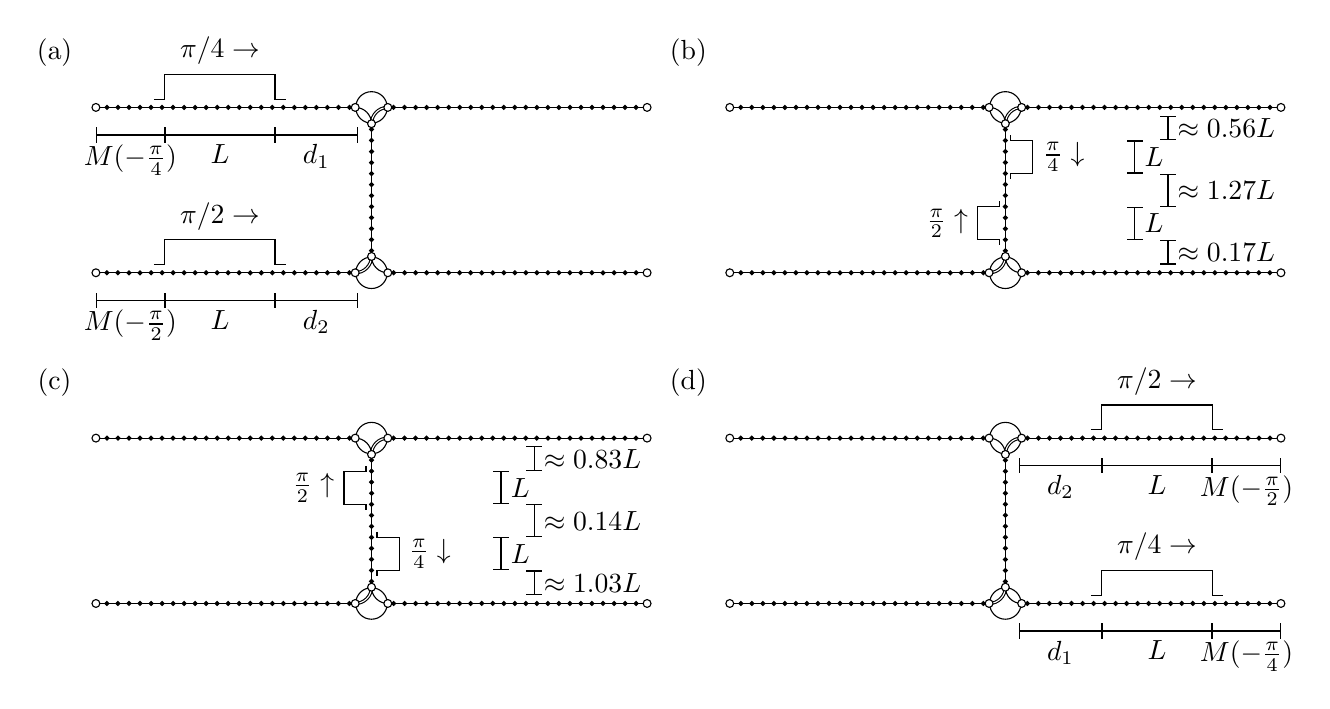
\begin{tikzpicture}[   scale=0.7,   
	dots/.style={circle,draw=black,fill=black,inner sep=0pt,minimum size=.5 mm}, 
	splitter/.style={circle,draw=black,fill=white,inner sep=0pt,minimum size=4mm},   
	attach/.style={circle,draw=black,fill=white,inner sep=0pt,minimum size=1mm}]
	
\begin{scope}[yshift= 6 cm]
  \node at (-.75,4) {(a)};

  \draw (0,0) to (10,0);   
  \draw (0,3) to (10,3);
  \foreach \x in {0,.2,.4,...,10}{
  \node at (\x, 0) [dots] {};
  \node at (\x, 3) [dots] {};
  }
  \foreach \y in {0,.2,.4,...,3}
  \node at (5,\y) [dots] {};
  
  \node (splitter42) at (5,0) [splitter] {};   
  \node (splitter41) at (5,3) [splitter] {};   
  \draw (splitter41.south) to (splitter42.north);      
  \draw (splitter41.west) to[out=0,in=90] (splitter41.south);   
  \draw[line width=1.2pt] (splitter41.south) to[out=90,in=180]           
  (splitter41.east);   
  \draw[line width=.4pt,white] (splitter41.south) to[out=90,in=180] (splitter41.east);
  \draw[line width=1.2pt] (splitter42.west) to[out=0,in=-90]           (splitter42.north);   
  \draw[line width=.4pt,white] (splitter42.west) to[out=0,in=-90]           (splitter42.north);   
  \draw (splitter42.north) to[out=-90,in=180] (splitter42.east);
  \node at (splitter41.east) [attach]{};
  \node at (splitter41.west) [attach]{};
  \node at (splitter41.south) [attach]{};
  \node at (splitter42.east) [attach]{};
  \node at (splitter42.west) [attach]{};
  \node at (splitter42.north) [attach]{};
  
  \node at (0,0) [attach]{};
  \node at (0,3) [attach]{};
  \node at (10,0) [attach]{};
  \node at (10,3) [attach]{};  

  \draw (1.05,3.15) to (1.25,3.15) to (1.25,3.6) to node[above]          
    {${\pi}/{4}\rightarrow$} (3.25,3.6) to (3.25,3.15) to (3.45,3.15);
  \draw (1.05,0.15) to (1.25,0.15) to (1.25,0.6) to node[above]          
    {${\pi}/{2}\rightarrow$} (3.25,0.6) to (3.25,0.15) to (3.45,0.15);
  \draw[|-|] (0,2.5) to node[below] {$M(-\frac{\pi}{4})$} (1.25,2.5);   
  \draw[|-|] (1.25,2.5) to node[below]{$L$}   (3.25,2.5);   
  \draw[|-|] (3.25,2.5) to node[below]{$d_1$} (4.75,2.5);
  \draw[|-|] (0,-.5) to node[below] {$M(-\frac{\pi}{2})$} (1.25,-.5);   
  \draw[|-|] (1.25,-.5) to node[below]{$L$}   (3.25,-.5);   
  \draw[|-|] (3.25,-.5) to node[below]{$d_2$} (4.75,-.5);
\end{scope}
  
%----------------------------------------------------------------------------------------%

\begin{scope}[xshift= 11.5cm, yshift=6cm]
  \node at (-.75,4) {(b)};

  \draw (0,0) to (10,0);   
  \draw (0,3) to (10,3);
  \foreach \x in {0,.2,.4,...,10}{
  \node at (\x, 0) [dots] {};
  \node at (\x, 3) [dots] {};
  }
  \foreach \y in {0,.2,.4,...,3}
  \node at (5,\y) [dots] {};
  
  \node (splitter42) at (5,0) [splitter] {};   
  \node (splitter41) at (5,3) [splitter] {};   
  \draw (splitter41.south) to (splitter42.north);      
  \draw (splitter41.west) to[out=0,in=90] (splitter41.south);   
  \draw[line width=1.2pt] (splitter41.south) to[out=90,in=180]           
  (splitter41.east);   
  \draw[line width=.4pt,white] (splitter41.south) to[out=90,in=180] (splitter41.east);
  \draw[line width=1.2pt] (splitter42.west) to[out=0,in=-90]           (splitter42.north);   
  \draw[line width=.4pt,white] (splitter42.west) to[out=0,in=-90]           (splitter42.north);   
  \draw (splitter42.north) to[out=-90,in=180] (splitter42.east);
  \node at (splitter41.east) [attach]{};
  \node at (splitter41.west) [attach]{};
  \node at (splitter41.south) [attach]{};
  \node at (splitter42.east) [attach]{};
  \node at (splitter42.west) [attach]{};
  \node at (splitter42.north) [attach]{};
  
  \node at (0,0) [attach]{};
  \node at (0,3) [attach]{};
  \node at (10,0) [attach]{};
  \node at (10,3) [attach]{};
  \begin{scope}[yshift = -10 cm]
    \draw (5.1,11.7) to (5.1,11.8) to (5.5,11.8) to node[right]          
      {$\frac{\pi}{4}\downarrow$} (5.5,12.4) to (5.1,12.4) to (5.1,12.5);
    \draw (4.9,11.3) to (4.9,11.2) to (4.5,11.2) to node[left]            
      {$\frac{\pi}{2}\uparrow$} (4.5,10.6) to (4.9,10.6) to (4.9,10.5);
    \draw[|-|] (7.95,12.85) to node[right] {$\approx 0.56L$} (7.95,12.4);   
    \draw[|-|] (7.35,12.4)  to node[right] {$L$}   (7.35,11.8);   
    \draw[|-|] (7.95,11.8)  to node[right] {$\approx 1.27L$} (7.95,11.2);   
    \draw[|-|] (7.35,11.2)  to node[right] {$L$}   (7.35,10.6);   
    \draw[|-|] (7.95,10.6)  to node[right] {$\approx 0.17L$} (7.95,10.15);
   \end{scope}  
\end{scope} 
  
%----------------------------------------------------------------------------------------%

  \node at (-.75,4) {(c)};

  \draw (0,0) to (10,0);   
  \draw (0,3) to (10,3);
  \foreach \x in {0,.2,.4,...,10}{
  \node at (\x, 0) [dots] {};
  \node at (\x, 3) [dots] {};
  }
  \foreach \y in {0,.2,.4,...,3}
  \node at (5,\y) [dots] {};
  
  \node (splitter42) at (5,0) [splitter] {};   
  \node (splitter41) at (5,3) [splitter] {};   
  \draw (splitter41.south) to (splitter42.north);      
  \draw (splitter41.west) to[out=0,in=90] (splitter41.south);   
  \draw[line width=1.2pt] (splitter41.south) to[out=90,in=180]           
  (splitter41.east);   
  \draw[line width=.4pt,white] (splitter41.south) to[out=90,in=180] (splitter41.east);
  \draw[line width=1.2pt] (splitter42.west) to[out=0,in=-90]           (splitter42.north);   
  \draw[line width=.4pt,white] (splitter42.west) to[out=0,in=-90]           (splitter42.north);   
  \draw (splitter42.north) to[out=-90,in=180] (splitter42.east);
  \node at (splitter41.east) [attach]{};
  \node at (splitter41.west) [attach]{};
  \node at (splitter41.south) [attach]{};
  \node at (splitter42.east) [attach]{};
  \node at (splitter42.west) [attach]{};
  \node at (splitter42.north) [attach]{};
 
  \node at (0,0) [attach]{};
  \node at (0,3) [attach]{};
  \node at (10,0) [attach]{};
  \node at (10,3) [attach]{};
  \begin{scope}[yshift = - 5cm]
  \draw (5.1,6.3) to (5.1,6.20) to (5.5,6.20) to node[right]            {$\frac{\pi}{4}\downarrow$} (5.5,5.6) to (5.1,5.6) to (5.1,5.5);
  \draw (4.9,6.7) to (4.9,6.8) to (4.5,6.8) to node[left]            {$\frac{\pi}{2}\uparrow$} (4.5,7.4) to (4.9,7.4) to (4.9,7.5);
  \draw[|-|] (7.95,7.85) to node[right] {$\approx 0.83L$} (7.95,7.4);   
  \draw[|-|] (7.35,7.4)  to node[right] {$L$}   (7.35,6.8);   
  \draw[|-|] (7.95,6.8)  to node[right] {$\approx 0.14L$} (7.95,6.2);   
  \draw[|-|] (7.35,6.2)  to node[right] {$L$}   (7.35,5.6);   
  \draw[|-|] (7.95,5.6)  to node[right] {$\approx 1.03L$} (7.95,5.15);
  \end{scope}
  
%----------------------------------------------------------------------------------------%
\begin{scope}[xshift=11.5cm]
  \node at (-.75,4) {(d)};

  \draw (0,0) to (10,0);   
  \draw (0,3) to (10,3);
  \foreach \x in {0,.2,.4,...,10}{
  \node at (\x, 0) [dots] {};
  \node at (\x, 3) [dots] {};
  }
  \foreach \y in {0,.2,.4,...,3}
  \node at (5,\y) [dots] {};
  
  \node (splitter42) at (5,0) [splitter] {};   
  \node (splitter41) at (5,3) [splitter] {};   
  \draw (splitter41.south) to (splitter42.north);      
  \draw (splitter41.west) to[out=0,in=90] (splitter41.south);   
  \draw[line width=1.2pt] (splitter41.south) to[out=90,in=180]           
  (splitter41.east);   
  \draw[line width=.4pt,white] (splitter41.south) to[out=90,in=180] (splitter41.east);
  \draw[line width=1.2pt] (splitter42.west) to[out=0,in=-90]           (splitter42.north);   
  \draw[line width=.4pt,white] (splitter42.west) to[out=0,in=-90]           (splitter42.north);   
  \draw (splitter42.north) to[out=-90,in=180] (splitter42.east);
  \node at (splitter41.east) [attach]{};
  \node at (splitter41.west) [attach]{};
  \node at (splitter41.south) [attach]{};
  \node at (splitter42.east) [attach]{};
  \node at (splitter42.west) [attach]{};
  \node at (splitter42.north) [attach]{};
 
  \node at (0,0) [attach]{};
  \node at (0,3) [attach]{};
  \node at (10,0) [attach]{};
  \node at (10,3) [attach]{};
  \draw (6.55,3.15) to (6.75,3.15) to (6.75,3.6) to node[above]            {${\pi}/{2}\rightarrow$} (8.75,3.6) to (8.75,3.15) to (8.95,3.15);
  \draw (6.55,.15) to (6.75,.15) to (6.75,.6) to node[above]            {${\pi}/{4}\rightarrow$} (8.75,.6)to (8.75,.15) to (8.95,.15);
  \begin{scope}[yshift=-.25cm]
  \draw[|-|] (5.25,2.75) to node[below] {$d_2$} (6.75,2.75);   
  \draw[|-|] (6.75,2.75) to node[below]{$L$}   (8.75,2.75);   
  \draw[|-|] (8.75,2.75) to node[below]{$M(-\frac{\pi}{2})$} (10,2.75);
  \draw[|-|] (5.25,-.25) to node[below] {$d_1$} (6.75,-.25);   
  \draw[|-|] (6.75,-.25) to node[below]{$L$}   (8.75,-.25);   
  \draw[|-|] (8.75,-.25) to node[below]{$M(-\frac{\pi}{4})$} (10,-.25);
  \end{scope}
\end{scope}
\end{tikzpicture} 
  \caption{This picture illustrates the scattering process for two wave packets that are incident on the input paths as shown in figure (a) at time $t=0$. Figure (b) shows the location of the two wave packets after a time $t_{A}={3L}/{2}$ and figure (c) shows the wave packets after a time $t_{B}=t_{A}+L$. After the particles pass one another they acquire an overall phase of $e^{i\theta}$. Figure (d) shows the final configuration of the wave packets after a total evolution time $t_{\mathrm{II}}={(Z+2d_{1}+L)}/{\sqrt{2}}$.}
  \label{fig:11_scattering_cartoon}
\end{figure}

Finally, we need to show the bound \eq{bound11}.  Unfortunately, this bound is slightly more difficult to prove, as we cannot naively use \lem{disconnected_MPQW}.  However, a more nuanced version of \lem{truncation} will allow us to approximate the evolution of both particles on $G'$ by the evolution on a disconnected graph for times less that $t_1$ and larger than $t_2$.  As such, we will only need to deal with the two-particle interactions for times between $t_1$ and $t_2$, and here we will be able to use \lem{truncation} to approximate the analysis by that on an infinite path for both the symmetric and anti-symmetric states.  Putting everything together, we have good approximations for all times $0 < t < t_{\CD}$, and thus we also have a good approximation for the final state.

\todo{determine correct vertex to remove (as it does depend on the momenta)}

To do this, let us define the graph $G^{\text{sep}}$ to be the $G'$ with the vertex labeled $(\lceil Z/2\rceil, 5)$ removed.  Note that $G^\text{sep}$ has four components, whereas $G'$ had three, but importantly that the two particles only have amplitude on separate components.  As such, we can then use \lem{disconnected_MPQW} and \lem{truncation} as in the case for any of the other logical computational basis states, at least for times in which the single-particle wave-packets remain far from the removed graph.  In particular, for all times $ 0 < t < t_1$, the approximation arising from the corresponding two-particle evolution on disconnected graphs (i.e., both the single-particle evolutions) remain a distance at least $L/3$ from the removed vertex.  Hence, using \lem{disconnected_MPQW} and the same single-particle evolutions as above, we have that
\begin{align}
  \Big\Vert e^{- i H_{G'}^{(2)} t_1} \ket{11_\text{in}} - T_1 T_2 \ket{\alpha_1^{1}(t_1)}\ket{\alpha_{1}^2 (t_1)} \Big\Vert \leq \xi_3 \sqrt{\frac{\log L}{L}}
\end{align}
for some constant $\zeta_5$.  In particular, we have that each of the individual single-particle evolutions an the finite-sized graphs have errors bounded by $\xi_1$ and $\xi_2$ times $\sqrt{\log L/L}$ (as in the above examples), and thus the two-particle evolution on $G^{\text{sep}}$ has an error bound with constant $\xi_1 + \xi_2$.  Another application of \lem{truncation}, using the fact that we are dealing with two-particles and thus the norm of $H_{G'}^{(2)}$ is bounded, the approximations are far from the removed vertex, and our bound on the error on $G^{\text{sep}}$ then gives the error as claimed.

At this point, our approximations to the time-evolved wavefunction are only supported on the long path far from the ends of the path, and thus we can use \lem{truncation} to look at the time-evolution on an infinite path.  This is exactly the point of \thm{two_particle_wavepacket_bound}, and we can thus use it's bounds.  It is at this point that we discover different evolutions for symmetric and anti-symmetric particles, as the relevant phase acquired during the overlap is dependent on the symmetry between the particles.

\todo{finish this part about the two-particle scattering}
In particular, if we as

After the two particles have moved passed each other and we have reach time $t_2$, we can use the same trick to approximate the time evolution for $t_2 < t < t_{\CD}$ as for the early times, and in particular we find that the error in our approximation for these times is bounded by the same value as for the early times.  Putting this together, we then have that
\begin{align}
  &\Big\Vert e^{- i H_G'^{(2)} t_{\CD}} \ket{11_{\text{in}}}^{1,2}_{\pm} - e^{i\theta_{\pm}} T_1^2 T_2^2 \ket{11_{\text{out}}}_{\pm}^{1,2}\Big\Vert\\
  & \qquad \leq \Big \Vert e^{-i H_G'^{(2)} t_{1}} \ket{\alpha_1^1(0),\alpha_2^1(0)}_{\pm}  - T_1T_2\ket{\alpha_1^1(t_1),\alpha_2^1(t_1)}_{\pm} \Big \Vert 
  + \Big \Vert e^{-i H_G'^{(2)} (t_2 - t_{1})}\ket{\alpha_1^1(t_1),\alpha_2^1(t_1)}_{\pm} - e^{i\theta_{\pm}}\ket{\alpha_1^1(t_2),\alpha_2^1(t_2)}_{\pm} \Big \Vert 
  + \Big \Vert e^{-i H_G'^{(2)} (t_{\CD}-t_{2})}\ket{\alpha_1^1(t_2),\alpha_2^1(t_2)}_{\pm} - T_1T_2\ket{\alpha_1^1(t_\CD),\alpha_2^1(t_\CD)}_{\pm} \Big \Vert\\
  & \qquad \leq \OO\big( \sqrt{\frac{\log L}{L}}\big)
\end{align}
and we have \eq{bound11}.
\end{proof}

At this point, we now understand how our assumed initial state propagates for single- and two-particle states, and we have the necessary building blocks for our universality result.  

\subsection{Explicit momenta}

Show that BH with momenta $\pi/2$ and $\pi/4$ with interaction strength $\sqrt{2} + 2$

%%%%%%%%%%%%%%%%%%%%%%%%%%%%%%%%%%%%%%%%%%%%%%%%%%%%%%%%%%%%%%%%%%%%%%%%%%
%  Multi-gate simulation
%

\section{Multi-gate simulation}

We now understand the single

\subsection{Many-particle single gate simulation}

\subsection{Combining gate simulations}

%%%%%%%%%%%%%%%%%%%%%%%%%%%%%%%%%%%%%%%%%%%%%%%%%%%%%%%%%%%%%%%%%%%%%%%%%%
%  Problem statement, and showing it is BQP-complete
%

\section{Universality via multi-particle scattering}




%%%%%%%%%%%%%%%%%%%%%%%%%%%%%%%%%%%%%%%%%%%%%%%%%%%%%%%%%%%%%%%%%%%%%%%%%%
%  Problem statement, and showing it is BQP-complete
%

\section{Extensions}

\subsection{Planar graphs}

%\subsection{

\section{Improvements and Modifications}


\subsection{Planar graphs}

%\subsection{

\section{Conclusions and open problems}

What about long-range interactions, but where the interactions die off?
Additionally, what about error correction?

smaller constants

\biblio{}

\end{document}